```latex
\subsection{Hyperparameter Analysis}

To improve the performance of the baseline transfer learning model, a multi-stage hyperparameter search procedure is conducted. All searches are implemented in \texttt{search.py} using grid search. Validation accuracy is used as the selection criterion throughout all experiments.

\subsubsection{Stage I: Coarse-Grained Hyperparameter Search}

In the first stage, we perform a coarse-grained search over optimizer type, backbone learning rate, classifier learning rate, weight decay, and batch size. The search space includes both SGD and AdamW optimizers, together with multiple learning rate and regularization configurations.

To analyze the influence of different hyperparameters, we visualize both correlation statistics and marginal distributions of validation accuracy.

\begin{figure}[H]
    \centering
    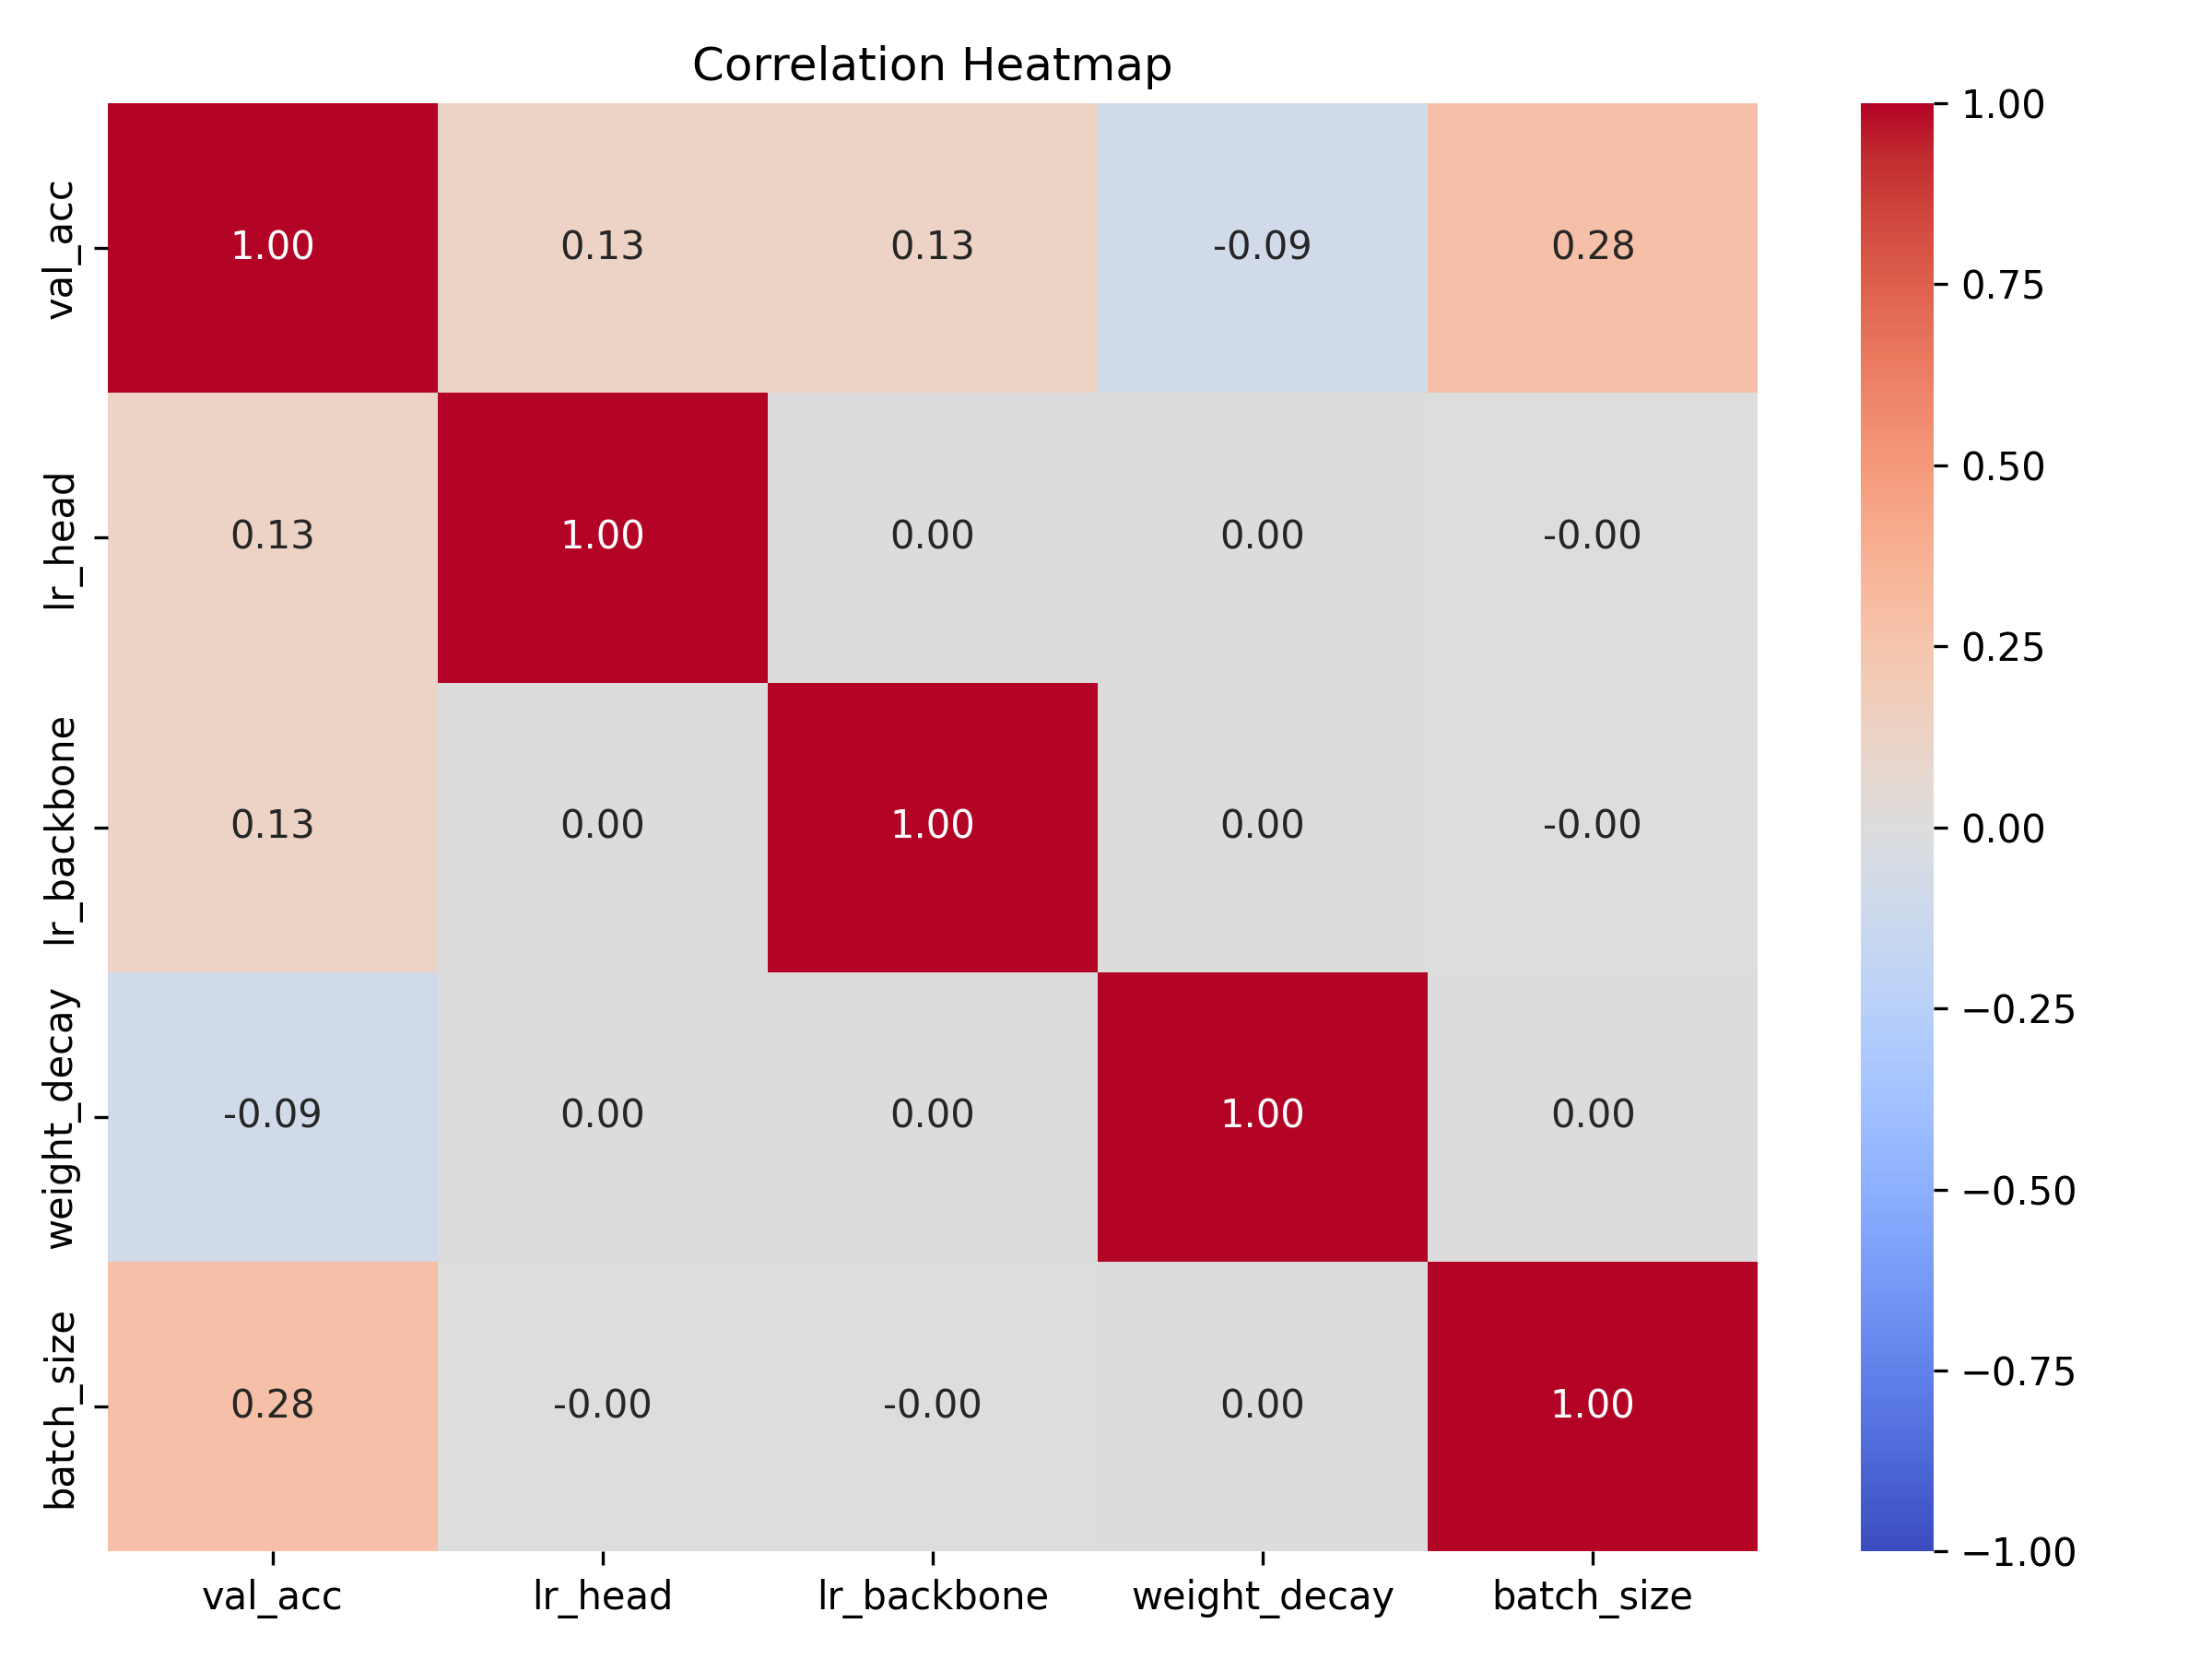
\includegraphics[width=0.8\textwidth]{figures/task1/stage_1_correlation_heatmap.png}
    \caption{Correlation coefficients between numerical hyperparameters and validation accuracy in Stage I search.}
    \label{fig:stage1_corr}
\end{figure}

\begin{figure}[H]
    \centering
    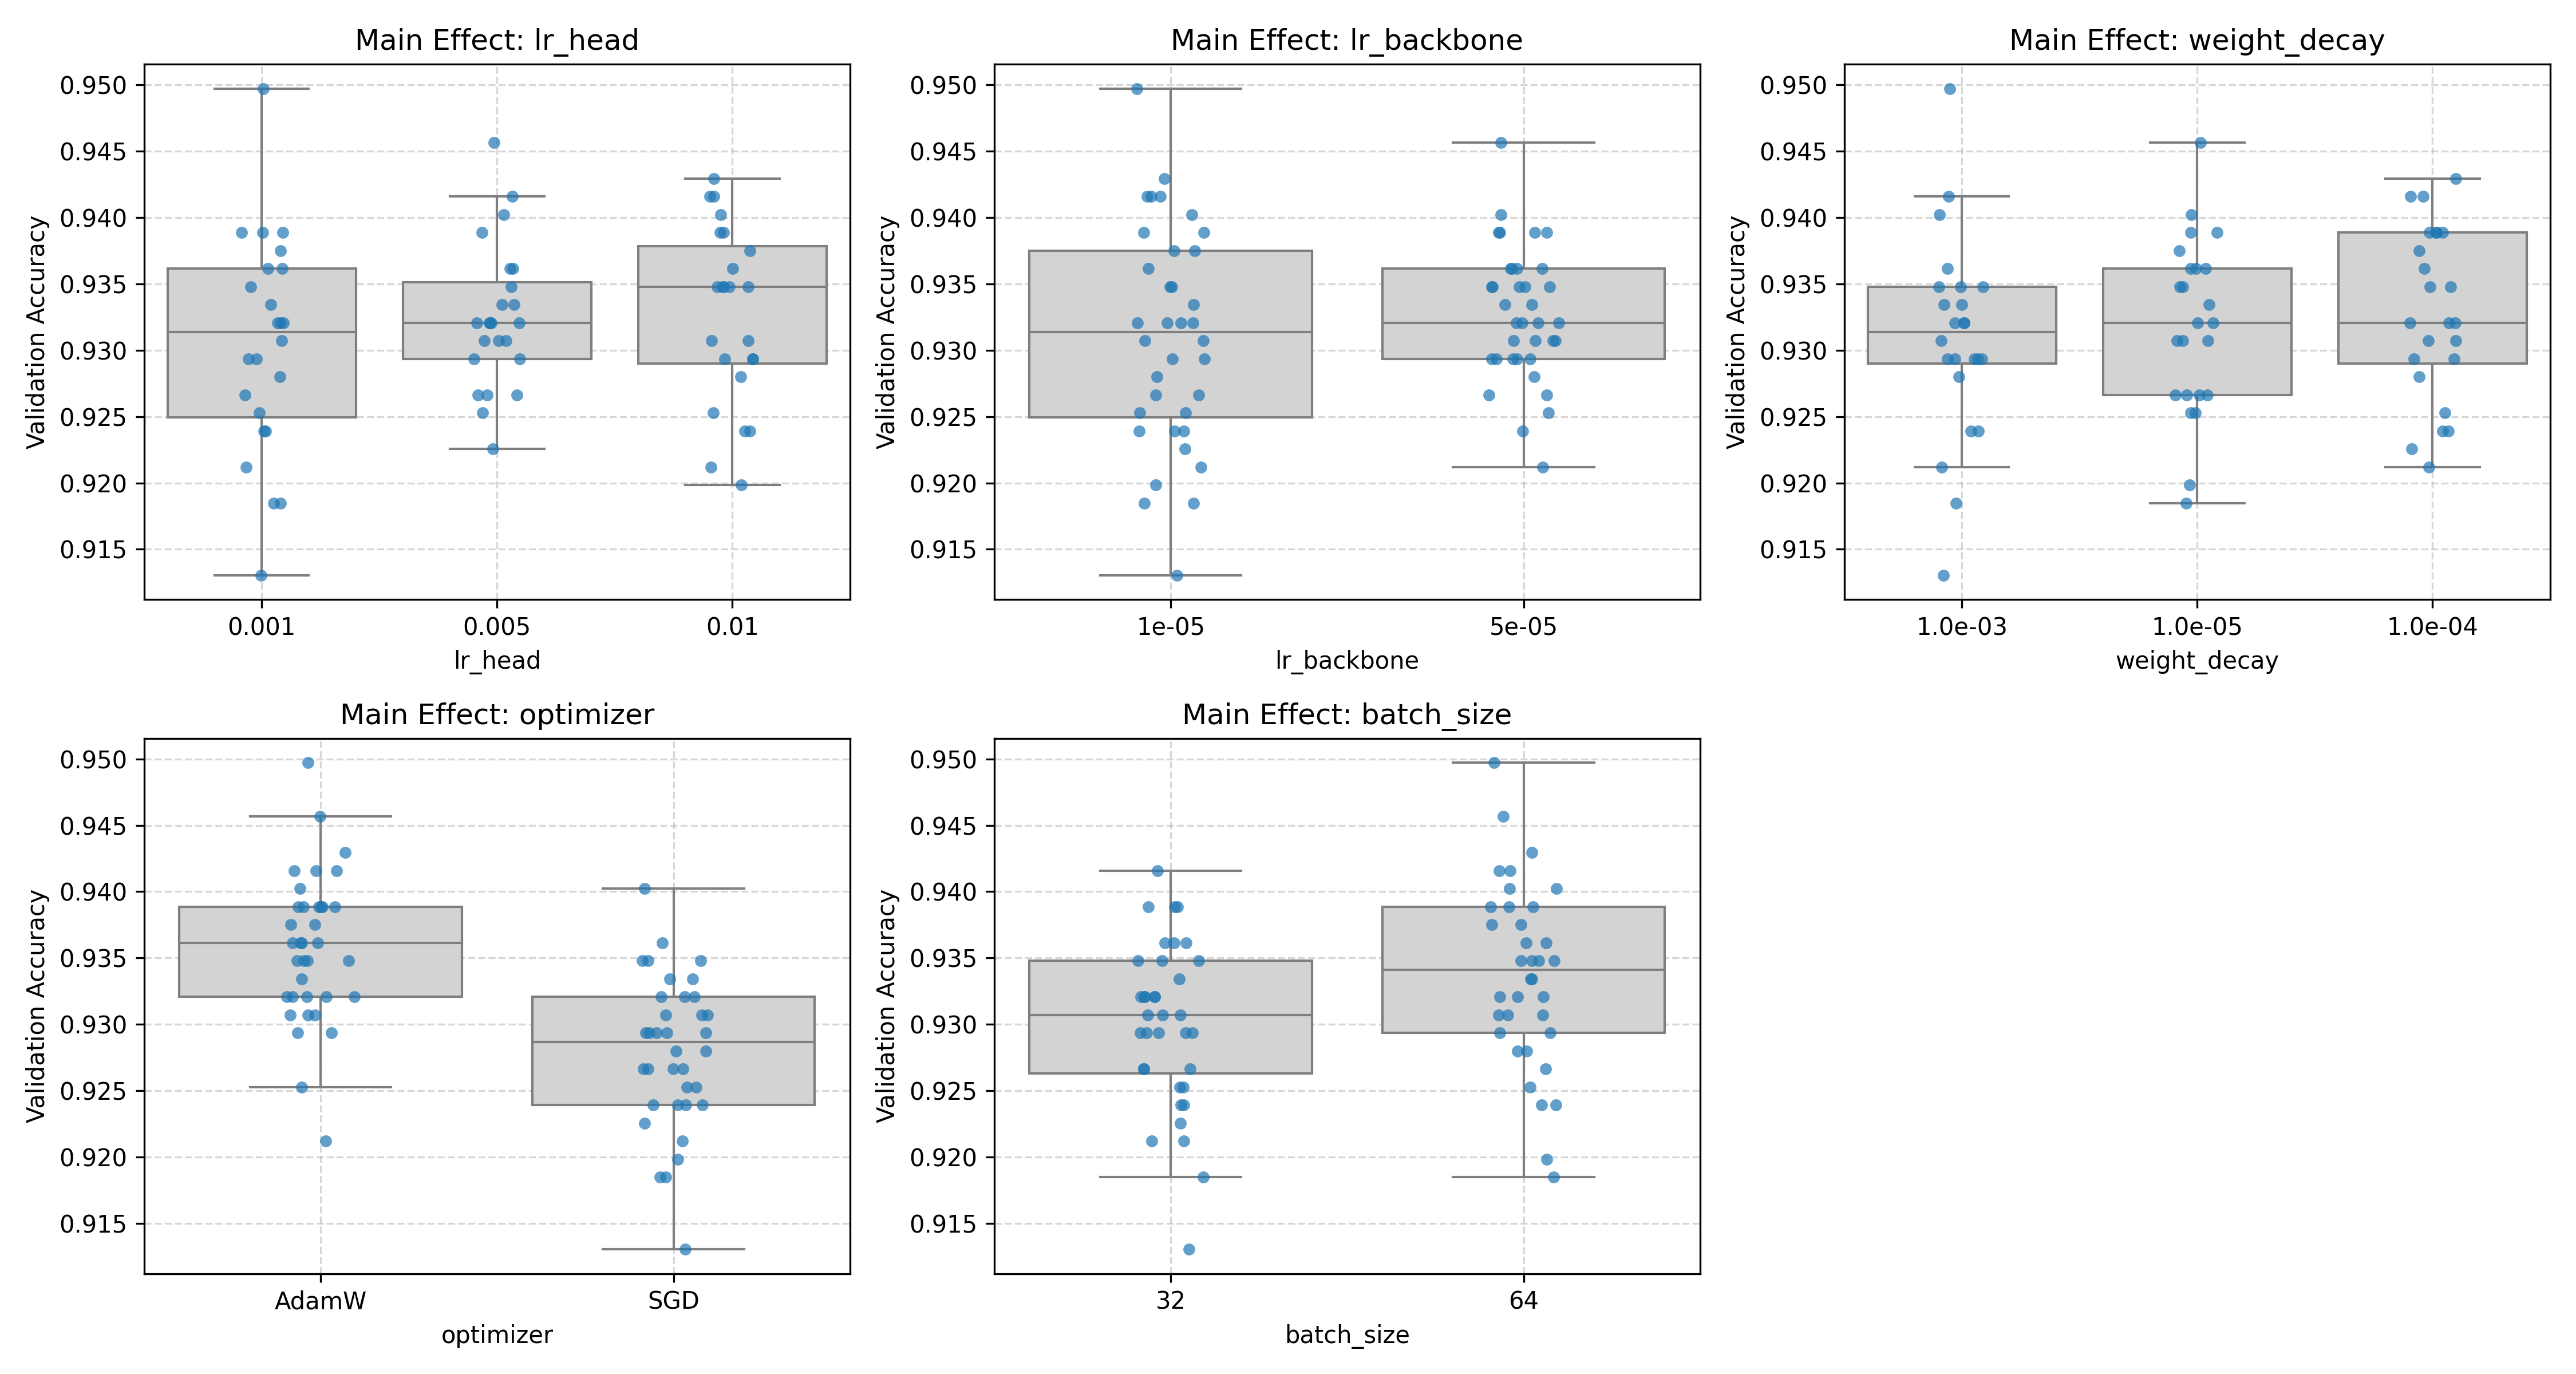
\includegraphics[width=0.8\textwidth]{figures/task1/stage_1_marginal_effects.png}
    \caption{Marginal effects of different hyperparameter choices in Stage I search.}
    \label{fig:stage1_marginal}
\end{figure}

The results show that batch size has the strongest correlation with validation accuracy, with a correlation coefficient of approximately 0.28. In particular, configurations with batch size 64 consistently outperform those with batch size 32. In addition, AdamW achieves noticeably better performance than SGD across most experiments.

The backbone learning rate and classifier learning rate both exhibit weak positive correlations with validation accuracy, while weight decay shows a weak negative correlation. However, these effects are significantly smaller compared with optimizer choice and batch size.

It should be noted that this analysis mainly considers marginal effects of individual hyperparameters and does not explicitly model interaction effects between variables. Nevertheless, the observed advantages of AdamW and larger batch size are sufficiently consistent across experiments.

\subsubsection{Stage II: Fine-Grained Search}

Based on the results of Stage I, AdamW and batch size 64 are fixed in the second stage. A more fine-grained grid search is then conducted over backbone learning rate, classifier learning rate, and weight decay.

The top three configurations obtained from the search are listed below:

\begin{table}[H]
\centering
\caption{Top configurations from Stage II hyperparameter search.}
\label{tab:stage2_top3}
\begin{tabular}{cccccc}
\toprule
Rank & $\text{lr}_{\text{head}}$ & $\text{lr}_{\text{backbone}}$ & Weight Decay & Optimizer & Batch Size \\
\midrule
1 & $2 \times 10^{-3}$ & $1 \times 10^{-5}$ & $1 \times 10^{-5}$ & AdamW & 64 \\
2 & $2 \times 10^{-3}$ & $2 \times 10^{-5}$ & $1 \times 10^{-5}$ & AdamW & 64 \\
3 & $1 \times 10^{-3}$ & $1 \times 10^{-5}$ & $1 \times 10^{-4}$ & AdamW & 64 \\
\bottomrule
\end{tabular}
\end{table}

\subsubsection{Epoch Sensitivity Analysis}

The top three configurations from Stage II are further evaluated under different training lengths of 30, 40, and 50 epochs.

\begin{table}[H]
\centering
\caption{Validation accuracy under different epoch settings.}
\label{tab:epoch_analysis}
\begin{tabular}{ccccc}
\toprule
Configuration & 30 Epochs & 40 Epochs & 50 Epochs \\
\midrule
Top 1 & 0.9524 & 0.9470 & 0.9511 \\
Top 2 & 0.9484 & 0.9429 & 0.9470 \\
Top 3 & 0.9538 & 0.9524 & 0.9484 \\
\bottomrule
\end{tabular}
\end{table}

The results indicate that extending training beyond 30 epochs does not provide additional improvement and may even slightly reduce validation accuracy, suggesting mild overfitting in later stages of training.

Finally, the third configuration trained for 30 epochs is selected as the final baseline setting:
\[
\text{optimizer} = \text{AdamW}, \quad
\text{lr}_{\text{backbone}} = 10^{-5}, \quad
\text{lr}_{\text{head}} = 10^{-3},
\]
\[
\text{weight decay} = 10^{-4}, \quad
\text{batch size} = 64, \quad
\text{epochs} = 30.
\]